\section{Variables and Constants}
\label{sec:vars}
\begin{frame}<beamer>
    \frametitle{Outline}
    \tableofcontents[currentsection]
\end{frame}

\begin{frame}[fragile]{Variable: valid identifiers (1)}
	\begin{itemize}
		\item {Consist of English letters (a-z, A-Z), numbers (0-9) and underscore (\_)}
		\item {Start with a letter (a-z, A-Z) or underscore (\_)}
		\item {Are case sensitive (\textbf{number} differs from \textbf{Number})}
		\item {Must not be reserved words (e.g \textcolor{blue}{int}, \textcolor{blue}{return})}
		\item {Check which are valid identifiers}
	\end{itemize}
	\begin{table}
	\begin{center}
		\begin{tabular}{|c|}
		\hline
		distance \\
		milesPerHour \\
		x-ray \\
		2ndGrade\\
		\$amount \\
		\_2nd \\
		two\&four \\
		\_hi \\
		return \\ \hline
		\end{tabular}
	\end{center}
	\end{table}
\end{frame}

\begin{frame}[fragile]{Variable: valid identifiers (1)}
	\begin{itemize}
		\item {Consist of English letters (a-z, A-Z), numbers (0-9) and underscore (\_)}
		\item {Start with a letter (a-z, A-Z) or underscore (\_)}
		\item {Are case sensitive (\textbf{number} differs from \textbf{Number})}
		\item {Must not be reserved words (e.g \textcolor{blue}{int}, \textcolor{blue}{return})}
		\item {Check which are valid identifiers}
	\end{itemize}
	\begin{table}
	\begin{center}
		\begin{tabular}{|c|c|}
		\hline
		distance & $\surd$\\ 
		milesPerHour & $\surd$\\
		x\textcolor{red}{-}ray & $\times$\\
		\textcolor{red}{2}ndGrade & $\times$\\
		\textcolor{red}{\$}amount & $\times$ \\
		\_2nd & $\surd$\\
		two\textcolor{red}{\&}four & $\times$\\
		\_hi & $\surd$\\
		\textcolor{red}{return} & $\times$\\ \hline
		\end{tabular}
	\end{center}
	\end{table}
\end{frame}

\begin{frame}[fragile]{Variable: valid identifiers (2)}
	\begin{itemize}
		\item {Recommended style}
		\begin{itemize}
			\item {Stay in one language (English recommended)}
			\item {Decide whether to use \underline{camel\textcolor{red}{C}ase\textcolor{red}{I}dentifiers} or \underline{snake\textcolor{red}{\_}case\textcolor{red}{\_}identifiers}}
			\item {When nesting blocks, indent every inner block by one additional tab!}
		\end{itemize}
	\end{itemize}
	\begin{lstlisting}[language=c, frame=none]
	#include <stdio.h>
	int main()
	{
	   float width = 3.0, height = 5.0, area = 0.0;
	   area = width*height;
	   printf("Area is: %f\n", area);
	   return 0;
	}
	\end{lstlisting}
\end{frame}

\begin{frame}[fragile]{Speaking identifiers}
	\begin{lstlisting}[language=c]
	/* calculate volume of square pyramid */
	int a, b, c;
	a = 3;
	b = 2;
	c = (1 / 3) * a * a * b;
	\end{lstlisting}
	\centering
	$\Downarrow$
	\begin{lstlisting}[language=c]
	/* calculate volume of square pyramid */
	int length, height, volume;
	length = 3;
	height = 2;
	volume = (1 / 3) * length * length * height;
	\end{lstlisting}
\end{frame}

\begin{frame}[fragile]{Constants}
	\begin{itemize}
		\item {Put key word `\textcolor{blue}{const}' before and type of variable definition}
		\item {The variable(s) become(s) constant(s)}
		\item {Constant means that you are not allowed to change the value after the definition}
	\end{itemize}
	\begin{lstlisting}[language=c, frame=none, numbers=none]
	const int a = 5, b = 6;
	const float c = 2.1;
	\end{lstlisting}
	\begin{lstlisting}[language=c]
	#include <stdio.h>
	int main()
	{
	    	const float PI = 3.14159;
	    	float r = 3.0, area = 0.0;
	    	PI = 3.14;   /*Invalid*/
	    	area = PI*r*r;   /*'area' has been updated here*/
	}
	\end{lstlisting}
	
\end{frame}

\begin{frame}[fragile]{Variables and Constants}
\begin{figure}
	\begin{center}
		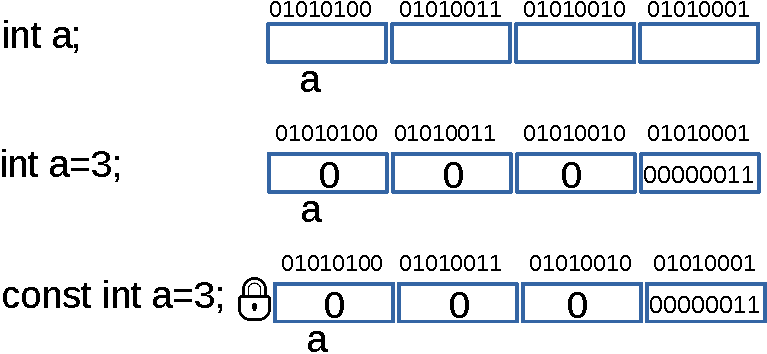
\includegraphics[width=0.8\linewidth]{figs/assign.pdf}
	\end{center}
\end{figure}
	
\end{frame}
